\documentclass{jsarticle}
\usepackage{bm}
\usepackage{amsmath}
\usepackage[dvipdfmx]{graphics}
\usepackage{here}
\usepackage[margin=20truemm]{geometry}
\usepackage{enumitem}
\renewcommand{\labelenumi}{【\arabic{enumi}】}
\renewcommand{\labelenumii}{(\arabic{enumii})}
\setlist[enumerate]{itemsep=10pt}

\begin{document}

\begin{center}
    {\huge 数理物理中間試験 予想問題集}\\
\end{center}

\begin{enumerate}
    \item 3次元空間に2つの質点A, Bがある。これらの質点の座標をそれぞれ$\bm{r}_A = (x_A,y_A,z_A), \bm{r}_B = (x_B,y_B,z_B)$とする時、これらが相対距離$r$に依存するポテンシャル$U(r)$により相互作用をしている。ただし$r$は以下のように定義する。

          $$
              \begin{aligned}
                  r & = \sqrt{(\boldsymbol{r}_A -\boldsymbol{r}_B})^2 \\
                    & = \sqrt{(x_A-x_B)^2+(y_A-y_B)^2+(z_A-z_B)^2}
              \end{aligned}
          $$

          質点の質量をどちらも$m$とする時、以下の問いに答えよ。

          \begin{enumerate}
              \item 2つの質点に働く力が、作用・反作用の法則を満たすことを示せ($x$成分のみ示せば良い)。
              \item この系の$x$方向の重心の運動量$p_x = m(\dot{x}_1 + \dot{x}_1)$が運動により保存することを示せ。

          \end{enumerate}

    \item 二次元平面上の質量$m$の質点があり、その座標を$(x,y)$とする。$r=\sqrt{x^2+y^2}$として、この質点が中心力$U(r)$を受けて運動している時、角運動量$L=m(y\dot{x} - x\dot{y})$が保存量であることを示せ。
    \item 図のように、摩擦の無い角度$\theta$の斜面上に質量$M$の物体があり、その質点と滑車を通じて質量$m$の物体が紐で繋がれてぶら下がっている。この2つの物体に働く力が釣り合っているとき、2つの質量の間に成り立つ条件を仮想仕事の原理を用いて求めよ。ただし紐は滑車によりなめらかに動くことができ、紐の重さは無視できるものとする。重力加速度は$g$とする。
          \begin{figure}[H]
              \centering
              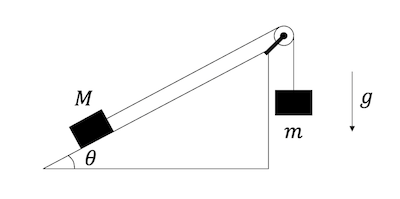
\includegraphics{fig/slope.png}
          \end{figure}
    \item 関数$f(x)$及びその微分$f'(x)$に依存する関数$F(f(x), f'(x))$を考える。ただし、$F$は$x$には陽に依存しない、すなわち $\partial F/\partial x = 0$ を満たすとする。この関数$F$についてオイラー・ラグランジュ方程式
          $$
              \frac{d}{dx} \left(\frac{\partial F}{\partial f'} \right)
              - \frac{\partial F}{\partial f} = 0
          $$
          が成り立っているとき、以下の量
          $$
              B = F - f' \frac{\partial F}{\partial f'}
          $$
          を考えると、
          $$
              \frac{dB}{dx} = 0
          $$
          を満たすことを示せ(ベルトラミの公式)。

          \newpage

    \item 二次元平面の原点に長さ$l$の棒に繋がれた質量$m$の質点がある。棒は原点を中心として摩擦なく自由に回転できる。また、棒は質量が無視でき、かつ運動により長さが変化しないものとする。棒が鉛直下方向からなす角度を$\theta$、重力加速度を$g$とする。この時、以下の問にこたえよ。
          \begin{enumerate}

              \item 角速度が$\dot{\theta}$である時、この系の運動エネルギーを求めよ。
              \item $\theta=0$の状態を基準とした時のこの系のポテンシャルエネルギーを求めよ。
              \item この系のラグランジアンを$\theta, \dot{\theta}$の関数として求め、オイラー・ラグランジュの式から運動方程式を導出せよ。ただし、結果は $\ddot{\theta} = $ の形に整理すること。
          \end{enumerate}

    \item 二次元空間において、質量$m$の質点が中心力$U(r)$を受けて運動をしている。ただし、質点の位置を$(x,y)$とした時、$r=\sqrt{x^2+y^2}$である。この質点の運動を、以下の極座標表示で表したい。

          $$
              \begin{aligned}
                  x & = r\cos \theta \\
                  y & = r\sin \theta
              \end{aligned}
          $$

          この時、以下の問に答えよ。
          \begin{enumerate}
              \item この系の運動エネルギー$K$を、$r, \theta, \dot{r}, \dot{\theta}$の関数として求めよ。
              \item この系のラグランジアンを求めよ。
              \item この系の運動を記述するオイラー・ラグランジュの方程式を書き下し、$r, \theta$が従う運動方程式を求めよ。
          \end{enumerate}

\end{enumerate}

\end{document}